\section{数据与网络}
\subsection{网络}
本案采用GraphQL 作为网络通讯的查询语言,GraphQL 三种操作:Query(查询)、Mutation(变更)
和 Subscription(订阅)。查询类似于RESTful API 中的GET方法,作用是从服务端获取一条或数条
记录而不更动服务端的任何状态,变更类似于RESTful API 中的 UPDATE、POST 和 DELETE 方法,对服务端
所管理的数据进行增加、修改、删除等操作。订阅操作是以流的形式建立客户端与服务端之间的长连接
使得客户端(本案中即Apollo Client)可以源源不断的受到服务端发送的数据。本案的网络协议
采用了GraphQL的默认实现,即查询和变更操作为HTTP、订阅操作为websocket。 在附录A中我们可以看到
表现层的Apollo Client对服务端进行访问时查询语句的详细定义。

而在业务层中,第四章已简述过各项服务的业务流程和功能。
这里再详细列出各个服务提供的schema。

\begin{center}
    \begin{longtable}{lcccccc}
        \caption{\label{schema}业务逻辑层 GraphQL Schema}                                                         \\
        \toprule
                       &      &      &                 &            & \multicolumn{2}{c}{身份权限}                \\
        \cmidrule{6-7}
        接口           & 服务 & 操作 & 输入            & 返回       & 管理员                       & 用户         \\
        \midrule
        \endfirsthead

        \toprule
                       &      &      &                 &            & \multicolumn{2}{c}{身份权限}                \\
        \cmidrule{6-7}
        接口           & 服务 & 操作 & 输入            & 返回       & 管理员                       & 用户         \\
        \midrule
        \endhead

        \bottomrule
        \endfoot
        class          & API  & 查询 & 班级ID          & 班级       & \yes                         & \yes         \\
        classes        & API  & 查询 & 无              & 所有班级   & \yes                         & \yes         \\
        executors      & API  & 查询 & 无              & 所有运行时 & \yes                         & \yes         \\
        user           & API  & 查询 & 用户ID          & 用户       & \yes                         & \yes         \\
        users          & API  & 查询 & 无              & 所有用户   & \yes                         &              \\
        station        & API  & 查询 & 车站ID          & 车站       & \yes                         & \yes         \\
        stations       & API  & 查询 & 无              & 所有车站   & \yes                         & \yes         \\
        instance       & API  & 查询 & 实例ID          & 实例       & \yes                         & \yes $^*$    \\
        instances      & API  & 查询 & 无              & 所有实例   & \yes                         & \yes $^*$    \\
        createStation  & API  & 变更 & 创建车站输入    & 车站       & \yes                         &              \\
        createExecutor & API  & 变更 & 创建运行时输入  & 运行时     & \yes                         &              \\
        createInstance & API  & 变更 & 创建实例输入    & 实例       & \yes                         & \yes $^\dag$ \\
        getUsers       & Auth & 查询 & 无              & 所有用户   & \yes                         &              \\
        createUser     & Auth & 变更 & 创建用户输入    & 用户       & \yes                         &              \\
        signUp         & Auth & 变更 & 注册输入        & 用户       & $\dag\dag$                   & $\dag\dag$   \\
        signIn         & Auth & 变更 & 登入输入        & JWT        & $\dag\dag$                   & $\dag\dag$   \\
        updatePwd      & Auth & 变更 & 修改密码输入    & 成功与否   & \yes                         & \yes         \\
        stationLayout  & Exec & 查询 & 实例ID          & 实例布局   & \yes                         & \yes$^*$     \\
        questions      & Exec & 查询 & 实例ID          & 考题       & \yes                         & \yes$^*$     \\
        instanceType   & Exec & 查询 & 实例ID          & 实例类型   & \yes                         & \yes$^*$     \\
        globalStatus   & Exec & 查询 & 实例ID          & 全局状态   & \yes                         & \yes$^*$     \\
        ping           & Exec & 查询 & 无              & pong       & \yes                         &              \\
        run            & Exec & 变更 & 实例ID          & 实例ID     & \yes                         & \yes $^*$    \\
        stop           & Exec & 变更 & 实例ID          & 实例ID     & \yes                         & \yes $^*$    \\
        createRoute    & Exec & 变更 & 实例ID+相应输入 & 实例ID     & \yes                         & \yes $^*$    \\
        cancelRoute    & Exec & 变更 & 实例ID+相应输入 & 实例ID     & \yes                         & \yes $^*$    \\
        manuallyUnlock & Exec & 变更 & 实例ID+相应输入 & 实例ID     & \yes                         & \yes $^*$    \\
        faultUnlock    & Exec & 变更 & 实例ID+相应输入 & 实例ID     & \yes                         & \yes $^*$    \\
        spawnTrain     & Exec & 变更 & 实例ID+位置     & 实例ID     & \yes                         & \yes $^*$    \\
        gameUpdate     & Exec & 订阅 & 实例ID          & 状态更新   & \yes                         & \yes $^*$    \\
    \end{longtable}
    \begin{itemize}
        \setlength{\itemsep}{0pt}
        \setlength{\parsep}{0pt}
        \setlength{\parskip}{0pt}
        \footnotesize
        \item[$*$] 仅返回该用户有权访问的查询或执行该用户有权执行的变更
        \item[$\dag$] 练习实例仅限
        \item[$\dag\dag$] 仅限未登录浏览器
    \end{itemize}
\end{center}

\subsubsection{网关}
本案采用 Apollo 提供的Apollo Federation 功能和 ApolloGateway 配置网关
如下:

\begin{lstlisting}
const gateway = new ApolloGateway({
  serviceList: [
    { name: 'auth', url: 'http://localhost:8001' },
    { name: 'api', url: 'http://localhost:8002' },
  ],
});
\end{lstlisting}

Apollo Federation 可以将多个GraphQL 服务器统合成一个GraphQL服务器向外暴露
服务。例如上代码所示,使用位于:8001端口的auth服务和位于:8002端口的api服务配置网关。



\subsection{数据库}
本案选用 ProsgreSQL 作为数据库管理系统,PostgreSQL是开源的对象-关系数据库数据库管理系统,
在类似BSD许可与MIT许可的PostgreSQL许可下发行。本案的SQL结构设计如图\ref{erd}:

\begin{figure}[htbp!]
    \centering
    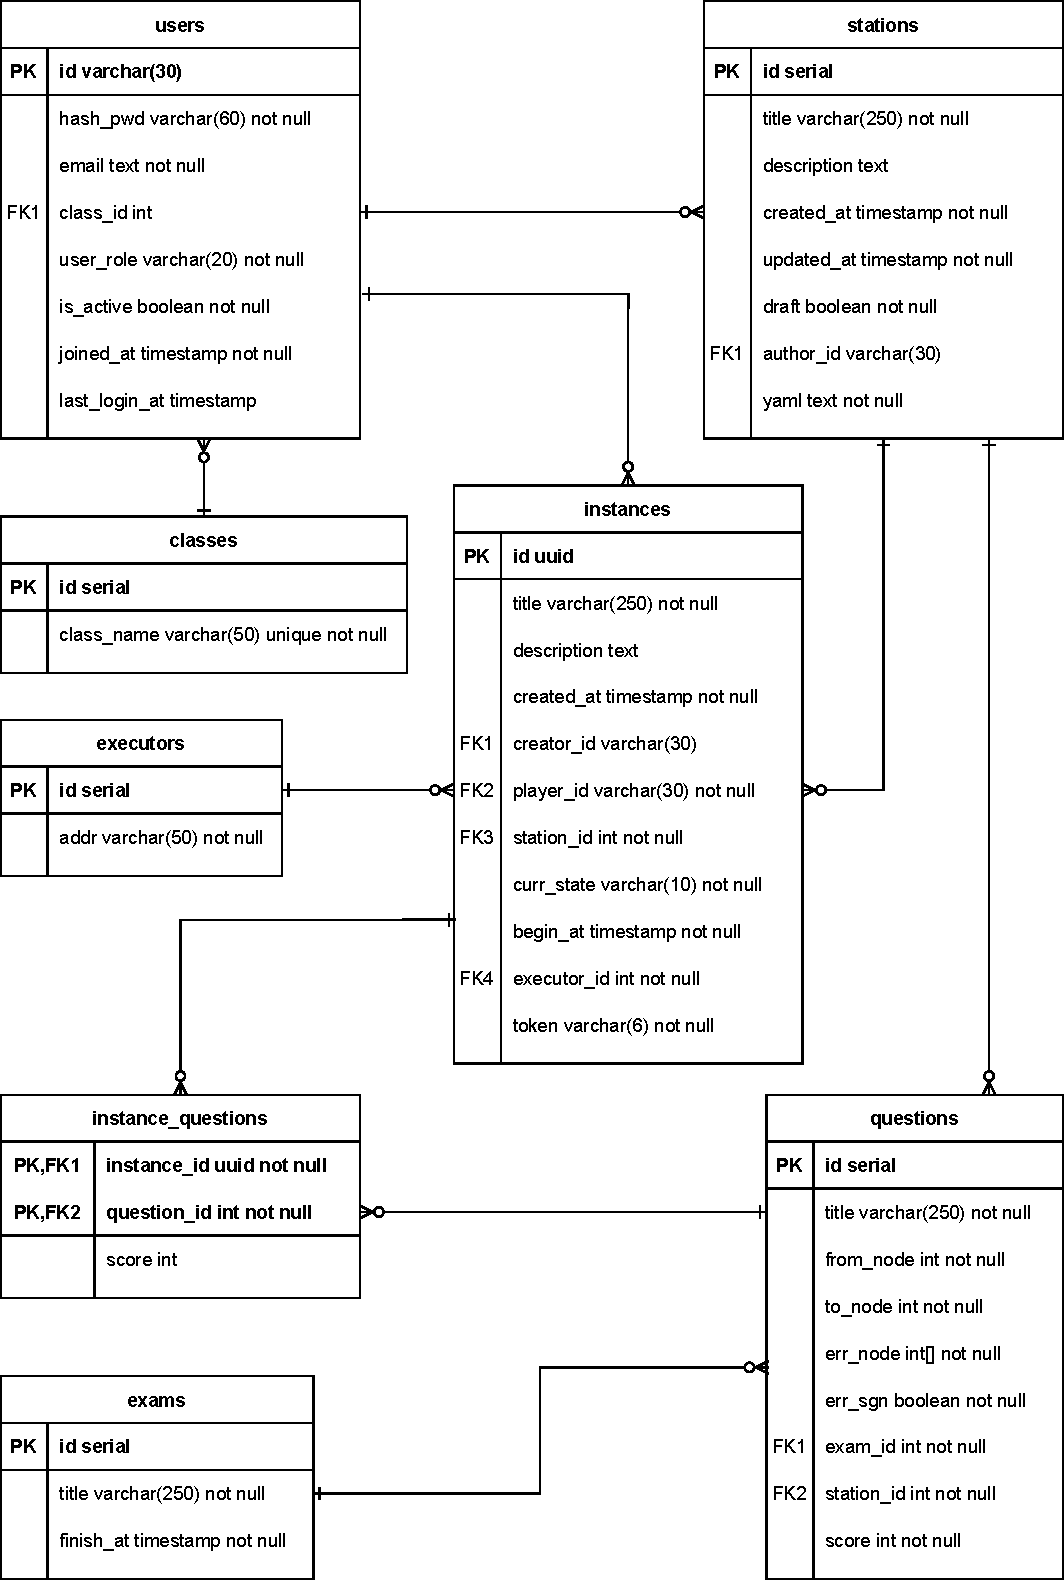
\includegraphics[width=0.95\textwidth]{figures/pdf/erd.pdf}
    \caption{\label{erd}数据库实体关系图}
\end{figure}

\subsubsection{表结构}

\paragraph 班级classes

\begin{lstlisting}
CREATE TABLE classes(
    id         serial       primary key,
    class_name varchar(50)  unique not null
)
\end{lstlisting}
主键id为自增整数,class\_name为班级名称

\paragraph 用户users

\begin{lstlisting}
CREATE TABLE users (
    id             varchar(30)     primary key,
    hash_pwd       varchar(60)     not null,
    email          text            not null,
    class_id       int  references classes(id) on delete set null,
    user_role      varchar(20)     not null,
    is_active      boolean         not null default 't',
    joined_at      timestamp       not null default now(),
    last_login_at  timestamp       default now()
)
\end{lstlisting}
解释:
\begin{itemize}
    \item 主键为id,类型为字符串,即用户自定义的用户id
    \item hash\_pwd 为加密后的用户密码
    \item email 为用户的电子邮箱地址
    \item class\_id 是表classes 的外键,表示用户所属的班级
    \item user\_role 表示用户角色
    \item is\_active 表示账户是否可用(未被禁用)
    \item joined\_at 和 last\_login\_at 默认是插入时的时间
\end{itemize}

\paragraph 车站stations

\begin{lstlisting}
CREATE TABLE stations (
  id          serial        primary key,
  title       varchar(250)  not null,
  description text,
  created_at  timestamp     not null default now(),
  updated_at  timestamp     not null default now(),
  draft       boolean       not null default 'f',
  author_id varchar(30) references users(id) on delete set null,
  yaml        text          not null
)
\end{lstlisting}
解释:
\begin{itemize}
    \item 主键为id, 自增整数
    \item title 为车站的标题
    \item description 为可空键,表示车站的备注
    \item draft 表示是否为草稿
    \item author\_id 是表 users 的外键,表示作者
    \item created\_at 和 updated\_at 默认是插入时的时间
    \item yaml 即为车站的描述文件内容
\end{itemize}

\paragraph 执行器executors

\begin{lstlisting}
CREATE TABLE executors (
    id             serial        primary key,
    addr           varchar(50)   not null
)
\end{lstlisting}
addr是该runtime的地址。

\paragraph 考试exams

\begin{lstlisting}
CREATE TABLE exams (
    id           serial        primary key,
    title        varchar(250)  not null,
    finish_at    timestamp     not null
)
\end{lstlisting}
finish\_at 表示结束时间,是考试实例特有的属性。

\paragraph 实例instances

\begin{lstlisting}
CREATE TABLE instances (
    id      uuid    primary key default gen_random_uuid(),
    title   varchar(250)  not null,
    description text,
    created_at  timestamp     not null  default now(),
    creator_id  varchar(30) references users(id) on delete ...,
    player_id   varchar(30)   not null  references users(id),    
    station_id  int           not null  references stations(id),
    curr_state  varchar(10)   not null,
    begin_at    timestamp     not null  default now(),
    executor_id int           not null  references executors(id),
    token       varchar(6)    not null
)
\end{lstlisting}
解释:
\begin{itemize}
    \item 主键为id, 类型是uuid\cite{group2020documentation}
    \item title 为实例标题
    \item curr\_state 表示实例当前的状态
    \item creator\_id 是表 users 的外键,表示创建者
    \item player\_id 是表 users 的外键,表示实例的用户
    \item created\_at  默认是插入时的时间
    \item begin\_at 表示实例的开始时间
    \item executor\_id 表示该实例的运行时id,是executors表的外键
    \item station\_id 是表 stations 的外键,表示实例的车站
    \item token 是游客令牌
\end{itemize}

\paragraph 问题questions

\begin{lstlisting}
CREATE TABLE questions (
    id          serial        primary key,
    title       varchar(250)  not null,
    from_node   int           not null,
    to_node     int           not null,
    err_node    int[]         not null,
    err_sgn     boolean       not null,
    exam_id     int           not null  references exams(id),
    station_id  int           not null  references stations(id),
    score       int           not null
)
\end{lstlisting}
解释:
\begin{itemize}
    \item from\_node 是本题目进路自何处
    \item to\_node 是本题目进路往何处
    \item err\_node 是本题目的预设故障结点
    \item err\_dgn 是本题目进路信号机是否出错
    \item exam\_id 是表 exams 的外键,表示本题目属于哪个考试
    \item station\_id 是表 stations 的外键,表示本题目属于哪个车站
    \item score 表示本道题赋分几何
\end{itemize}

\paragraph 实例问题(即“考题”)instance\_questions

\begin{lstlisting}
CREATE TABLE instance_questions (
    instance_id    uuid   not null references instances(id),
    question_id    int    not null references questions(id),
    score          int,
    PRIMARY KEY (instance_id, question_id)
)
\end{lstlisting}

本表使用instance\_id和question\_id两个外键作为联合主键,本表的一个记录表示
某个实例(必然为考试实例)的某个题目得分几何。score是可空的,因为在新建考试实例的
时候就会在本表中新建进路,在完成某道考题的时候更新记录。

\subsection{持久层}
\subsubsection{ORM}
本案采用ORM以提升开发效率,ORM 是一种程序设计技术,用于将数据库的记录映射到程序语言的对象中,
或者将对象映射到某个表中,其封装了CRUD的SQL语句操作,可以让开发者从表中直接读入一个对象。或者将
一个对象插入某个表。效果上说,它其实是创建了一个可在编程语言里使用的“虚拟对象数据库”。

在本案的持久层 uroj-db 中,定义了程序的DAO层逻辑,封装了所有项目需要的数据库访问方法。
以便供Api, Auth, Executor 等服务复用。uroj采用diesel作为本案的ORM库,
将DAO层的各种结构体定义和上小结所定义的SQL表映射起来的,
就是diesel client所生成的schema。

这里简单介绍一下 diesel 的使用步骤。首先需要定义migration,migration可以简单理解为创建和删除表
的sql文件。将上一节的表定义好后。使用diesel生成schema,schema是diesel使用
rust macro定义的一些字段。之后我们需要定义DAO层的struct,对于一个表一般而言需要两种
struct,一个是读取用一个是插入用,但需要derive diesel提供的相应的过程宏,这样就可以
将sql表和DAO 层 struct映射起来,再使用diesel提供的方法进行CRUD操作。

\subsubsection{连接池}
连接池(英语:connection pool)是维护的数据库连接的缓存,
以便在将来需要对数据库发出请求时可以重用连接。
每次需要再打开一个新的数据库连接都是低效的,而且在高流量条件下会导致资源耗尽。
可以使用连接池解决这个问题以提高在数据库上执行命令的性能\cite{zhong2005database}。
为每个用户打开和维护数据库连接,尤其是对动态数据库驱动的网站应用程序发出的请求,
既昂贵又浪费资源。在连接池中,创建连接之后,将连接放在池中并再次使用,这样就不必创建新的连接。
如果所有连接都正在使用,则创建一个新连接并将其添加到池中。
连接池还减少了用户必须等待创建与数据库的连接的时间。

uroj 采用 r2d2 作为数据库连接池,r2d2 是rust的一个通用连接池。
r2d2对于它所管理的连接类型是不可知的。
ManageConnection特性的实现者提供了数据库特定的逻辑来创建和检查连接的健康状况。

在 uroj-db crate 中使用如下create\_connection\_pool函数创建一个连接池。在
uroj-api 和 uroj-runtime 使用本函数创建连接池。
\begin{lstlisting}
use diesel::r2d2::{ConnectionManager, Pool};
use diesel::{pg::PgConnection, r2d2::PooledConnection};

pub type PgPool = Pool<ConnectionManager<PgConnection>>;
pub type Conn =
         PooledConnection<ConnectionManager<PgConnection>>;

pub fn create_connection_pool() -> PgPool {
    let url = env::var("DB_URL").expect("Can't get DB URL");
    let manager = ConnectionManager::<PgConnection>::new(url);
    Pool::builder()
        .build(manager)
        .expect("Failed to create pool")
}
\end{lstlisting}

\subsubsection{时区处理}
本项目从数据库PostgreSQL、业务逻辑层到前端的表现层,一个需要重视的问题是时区。
若是单时区应用的话大可以直接在数据库中保存北京时间的字符串,但本案为了保证通用性
,考虑来自不同时区的用户,或者是部署于不同时区的数据库、服务器。因此在PostgreSQL中,
本例使用时间戳(timestamp)保存时间,时间戳是UTC1970年1月1日0时0分0秒起至现在的总秒数。
因此是一种没有时区的信息,或者说是协调世界时0时区的时间。

从数据库中取到的时间戳,在业务逻辑层中被表示为 chrono 库中的 NaiveDateTime,NaiveDateTime是
一种没有时区的日期时间字面量,其可以被简单地转换成任何时区的DateTime,因此我们会在
业务逻辑层中将0时区的时间戳转换成业务逻辑层服务器所在时区的时间,并呈递给表现层。表现层
显示哪种时区完全取决于其访问部署于何处的服务器。
